\documentclass[hidelinks, 12pt, a4paper]{article}

\usepackage{tabularx} %full-width tables
\usepackage{moresize} %Huge and HUGE
\usepackage[margin=0in]{geometry}%Margins
\usepackage[none]{hyphenat}%Remove hyphenation
\usepackage{enumitem}%to set gaps in itemize
\usepackage{fontawesome}
\usepackage{hyperref}
\usepackage{blindtext}
\usepackage{xcolor}
\usepackage{afterpage}
\usepackage{tikz}
\usepackage[skins]{tcolorbox}
\usepackage{xcolor}

\usepackage{multicol}

\usepackage[sfdefault,light]{roboto}

%\cellwidth in tabularx size
\makeatletter
\newcommand\cellwidth{\TX@col@width}
\makeatother

\definecolor{sidebarColor}{HTML}{001C5E}
\definecolor{skillBackground}{HTML}{98A0B2}
\definecolor{skillForeground}{HTML}{EBA500}

%Right-aligned tabularx
\newcolumntype{R}{>{\raggedleft\arraybackslash}X}

%No page numbering
\pagenumbering{gobble}

\newcommand{\smitem}[1]{\item {\small {#1}}}

\newenvironment{bullets}{\begin{minipage}[t]{\linewidth}\begin{itemize}[leftmargin=2em,label=-,nosep]}{\end{itemize}\end{minipage}\vspace{2pt}}

\newenvironment{sectionitem}{\vspace{6pt}\noindent\tabularx{\linewidth}{p{70pt}X}}{\endtabularx}

\newcommand{\tech}[1]{
	\tcbox[skin=enhanced,nobeforeafter,colframe=black!20,size=fbox,height=15pt]{\footnotesize#1}
}

\newcommand{\darktech}[1]{
	\tcbox[skin=enhanced,nobeforeafter,colback=black!10,colframe=black!30,size=fbox,height=15pt]{\footnotesize#1}
}

\newcommand{\sectionheader}[1]{
	\vspace{6pt}
	{
		\noindent
		\hspace{3pt}
		%\fontfamily{lmr}\selectfont
		\Large\textbf{#1}}}

\begin{document}
	\noindent\fcolorbox{sidebarColor}{sidebarColor}{%
		\color{white}
		\begin{minipage}{\dimexpr0.35\textwidth-2\fboxrule-2\fboxsep\relax}
			\vspace{4pt}
			\begin{center}
				\begin{tikzpicture}
				\color{black}
				\node[circle,draw,inner sep=40pt,fill overzoom image=picture] (A) {};
				\end{tikzpicture}\\
				
				\vspace{12pt}
				
				\textbf{
					\LARGE Steven Lowes
				}
				\vspace{8pt}
				
				\begin{tabular}{rc}
					Durham, UK                                                     & \faHome                                                       \\
					\href{mailto:cv@stevenlowes.com}{cv@stevenlowes.com}           & \href{mailto:cv@stevenlowes.com}{\faEnvelope}                 \\
					\href{https://www.linkedin.com/in/steven-lowes/}{steven-lowes} & \href{https://www.linkedin.com/in/steven-lowes/}{\faLinkedin} \\
					\href{https://github.com/motherlymuppet}{motherlymuppet}       & \href{https://github.com/motherlymuppet}{\faGithub}           \\
					\href{http://www.stevenlowes.com}{stevenlowes.com}             & \href{http://www.stevenlowes.com}{\faLink}                    \\
				\end{tabular} \\
				
				\vspace{12pt}
				
				\begin{minipage}{0.9\linewidth}
					\begin{center}
						\begin{Large}
							\textbf{Summary}
						\end{Large}
					\end{center}
				
								\vspace{-12pt}
					
					Third year Durham University Computer Science student
					
					\vspace{8pt}
					
					Self-directed, efficient generalist, able to quickly learn new technologies with a desire to work on challenging problems
					
					\vspace{8pt}
					
					Creative, unorthodox, and innovative, able to think outside the box to find the best solution.
					
					\vspace{8pt}
					
					Proficient public speaker with great communication in teams and plenty of leadership experience
					
					\vspace{8pt}
					
					Back-end development preferred, but happy to do some front-end. 
					
					\vspace{8pt}
					
					\begin{center}
						\begin{Large}
							\textbf{Career Interests}
						\end{Large}
					\end{center}
				
					\vspace{-8pt}
					
					Startups and small teams with flat hierarchy, in North-East England or Remote. \textbf{Areas of Interest include:}
					
					\vspace{8pt}
			
				\begin{bullets}
					\smitem{Automation (Home/Industrial)}
					\smitem{FinTech}
					\smitem{Data Science}
					\smitem{High Performance Computing}
					\smitem{Embedded Systems}
				\end{bullets}
			
					\begin{center}
						\begin{Large}
							\textbf{Skills}
						\end{Large}
					\end{center}
				
				\vspace{-8pt}
				\emph{I am the go-to guy regarding:}
				
				\darktech{Java} \darktech{Kotlin} \darktech{SQL} \darktech{Excel}
				
				\emph{I can teach you about:}
				
				\darktech{Python} \darktech{JS} \darktech{C\#} \darktech{NodeJS} \darktech{APIs} \darktech{LaTeX} \darktech{Concurrency} \darktech{Optimisation} \darktech{Electronics} \darktech{CPU Design} \darktech{Business}
				
				\emph{I also have experience with:}
				
				\darktech{HPC} \darktech{GPGPU} \darktech{NoSQL} \darktech{Typescript} \darktech{C} \darktech{Haskell} \darktech{MATLAB} \darktech{Prolog}
				\end{minipage}
			\end{center}
		\end{minipage}
	}
	\hspace{0.02\textwidth}
	\begin{minipage}{0.58\textwidth}	
		
		\sectionheader{Education}
		
		\begin{sectionitem}
			2016 --- 2019&\textbf{\href{https://www.dur.ac.uk/}{Durham University}} (\href{https://www.dur.ac.uk/trevelyan.college/}{Trevelyan College})\\
			\emph{Durham}&\href{https://www.dur.ac.uk/courses/info/?id=11509\&title=Computer+Science\&code=G400\&type=BSC\&year=2016}{BSc Computer Science}\\
			&\begin{bullets}
				\smitem{Expected: 1st Class (Hons)}
			\end{bullets}\\
			2015 --- 2016&\href{https://www.dur.ac.uk/courses/info/?id=11558\&title=General+Engineering\&code=H100\&type=MENG\&year=2015}{MEng General Engineering}\\
			&\begin{bullets}
				\smitem{Year 1: 2:2 Equivalent}
				\smitem{Module - \href{https://www.dur.ac.uk/faculty.handbook/module_description/?module_code=COMP1011}{\emph{Introduction to Programming}: \textbf{89\%}}\\Convinced me to switch course}
			\end{bullets}\\
		\end{sectionitem}
		
		\begin{sectionitem}
			2008 --- 2015&\textbf{\href{http://www.parkviewlearning.net/}{Park View School}}\\
			\emph{Co. Durham}&\begin{tabularx}{250pt}{XX}
				A-Levels:&GCSEs:\\
			\end{tabularx}\\
			&\begin{tabularx}{250pt}{XX}
				\begin{bullets}
					\smitem{Business - A*}
					\smitem{Maths - A}
					\smitem{Physics - B}
				\end{bullets}&
				\begin{bullets}
					\smitem{3 $\times$ A*}
					\smitem{7 $\times$ A}
					\smitem{1 $\times$ B, C}
				\end{bullets}\\
			\end{tabularx}\\
		\end{sectionitem}
		
		\vspace{-12pt}
		
		\sectionheader{Work}
		
		\begin{sectionitem}
			Oct 2018&\textbf{Lab Demonstrator}\\
			--- Present& Durham University\\
			\emph{Durham}& \begin{bullets}
				\smitem{Ran sessions to support students' learning}
				\smitem{Covering: Electronics, Machine Architecture, Operating Systems, Databases, and Networks}
			\end{bullets}\\
		\end{sectionitem}
	
		\vspace{4pt}
		
		\begin{sectionitem}
			July ---&\textbf{Junior Software Engineer (Internship)}\\
			Oct 2018& \href{https://www.condecoconnect.com/}{Condeco Group Ltd.}\\
			\emph{Newcastle}& \begin{bullets}
				\smitem{Full-Stack web development with microservices}
				\smitem{Focus on backend API development}
				\smitem{Designed and pitched a new microservice}
			\end{bullets}\\
			&\tech{ASP.net Core} \tech{Typescript} \tech{Android} \tech{Azure} \tech{SQL}\\
		\end{sectionitem}
		
		\begin{sectionitem}			
			March ---&\textbf{Full Stack Developer}\\
			May 2017&\href{http://planforprobate.com/}{Plan for Probate (North) Ltd.}\\
			\emph{Co. Durham}&\begin{bullets}
				\smitem{Developed an online CRM portal tracking payments and customer information}
				\smitem{Employed an Agile framework to keep clients informed throughout the consulting process}
			\end{bullets}\\
			&\tech{Java} \tech{JSP} \tech{SQL} \tech{JS} \tech{Google Cloud Platform}\\
		\end{sectionitem}
		
%		\begin{sectionitem}
%			July ---&\textbf{Java Programmer}\\
%			Oct 2016&\href{https://www.facebook.com/tripefactory.sunderland/}{E. Hall Tripe \& Poultry Ltd.}\\
%			\emph{Sunderland}&\begin{bullets}
%				\smitem{Developed a logistics system which creates packing lists for the drivers, and calculates delivery routes, previously done manually}
%			\end{bullets}\\
%			&\tech{Java} \tech{Swing} \tech{SQL}\\
%		\end{sectionitem}
		
		\begin{sectionitem}
			2013 ---&\textbf{Data Analyst}\\
			2017&\href{http://www.lowes.co.uk}{Lowes Financial Management}\\
			\emph{Newcastle}&\begin{bullets}
				\smitem{Created data analysis tools which produce data and graphs used in product brochures}
			\end{bullets}\\
			&\tech{Java} \tech{SQL} \tech{Excel} \tech{VBA}\\
		\end{sectionitem}
		
		\sectionheader{Accomplishments}
		
		\vspace{4pt}
		
		\begin{bullets}
			\smitem{Won the GitHub Prize for Best Dev Tool in \href{https://durhack.com}{Durhack 2018}, overall runner-up with \href{https://github.com/motherlymuppet/sharpshot}{\emph{SharpShot}}, an esoteric visual programming language}
			\smitem{BAE Systems \emph{Capture the Flag} Runner-Up 2017}
			\smitem{Active GitHub account, contributing to FOSS}\\
			\smitem{Chair of the committee that governs extracurricular student groups, \href{https://www.thebubble.org.uk/current-affairs/student-life/motion-voted-down-by-outraged-assembly/}{successfully campaigning for more student consultation}}
			\smitem{Represent over 4,000 students as Science Faculty Rep, speaking publicly and lobbying senior leadership regarding student issues}
			\smitem{Held leadership positions on five student groups \& president of two}\\
			\smitem{Actively involved with \href{http://community.dur.ac.uk/dur.improv/}{Shellshock! Improvised Comedy}, performing in a \href{https://tickets.edfringe.com/whats-on/here-be-improv}{sell-out show at Edinburgh Fringe in 2018}}
			\smitem{\href{https://i.imgur.com/4Uz2USm.jpg}{I made a super cool electric bike (click)}}
		\end{bullets}
	\end{minipage}
	
	\newpage
	
	\vspace*{12pt}
	
	\begin{center}
		\Huge \textbf{Portfolio}
	\end{center}
	
	\hspace{0.02\textwidth}
	\begin{minipage}{0.40\textwidth}		
		\begin{center}
			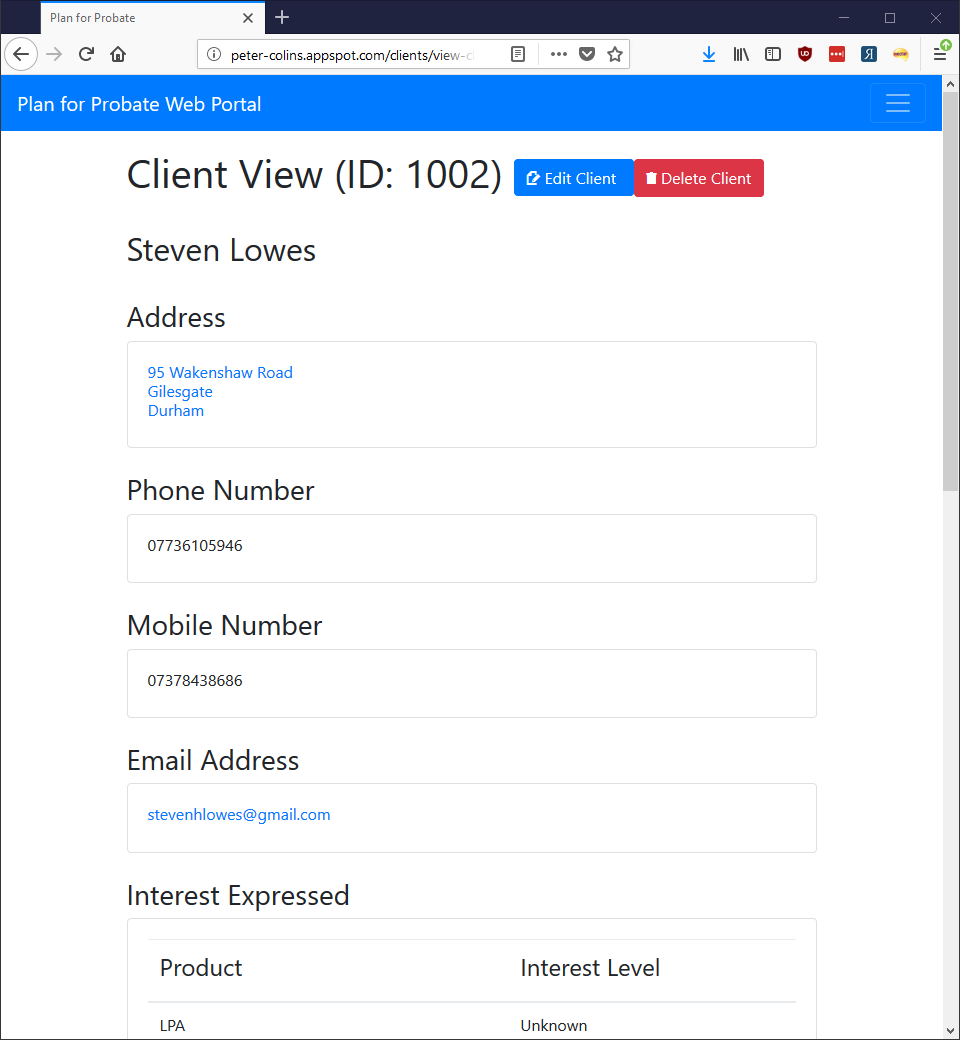
\includegraphics[width=0.9\linewidth]{planforprobate.png}
		\end{center}
		\textbf{Plan For Probate Web Portal} (May 2017)
		
		Plan For Probate's internal web portal. Tracks clients, and tasks currently in progress. Allows for file upload and storage for important documents. Secured using Google Login, and Database encrypted to comply with GDPR. Used by the company to store and manage all ongoing tasks and client information. The web portal has replaced the previous system which used index cards to track their clients, decreasing the time spent on admin and number of errors/missed appointments.
		
		\tech{Java} \tech{SQL} \tech{JSP} \tech{Bootstrap} \tech{Javascript} \tech{Google Cloud Platform}
		
		\begin{center}
			\href{https://github.com/motherlymuppet/sharpshot}{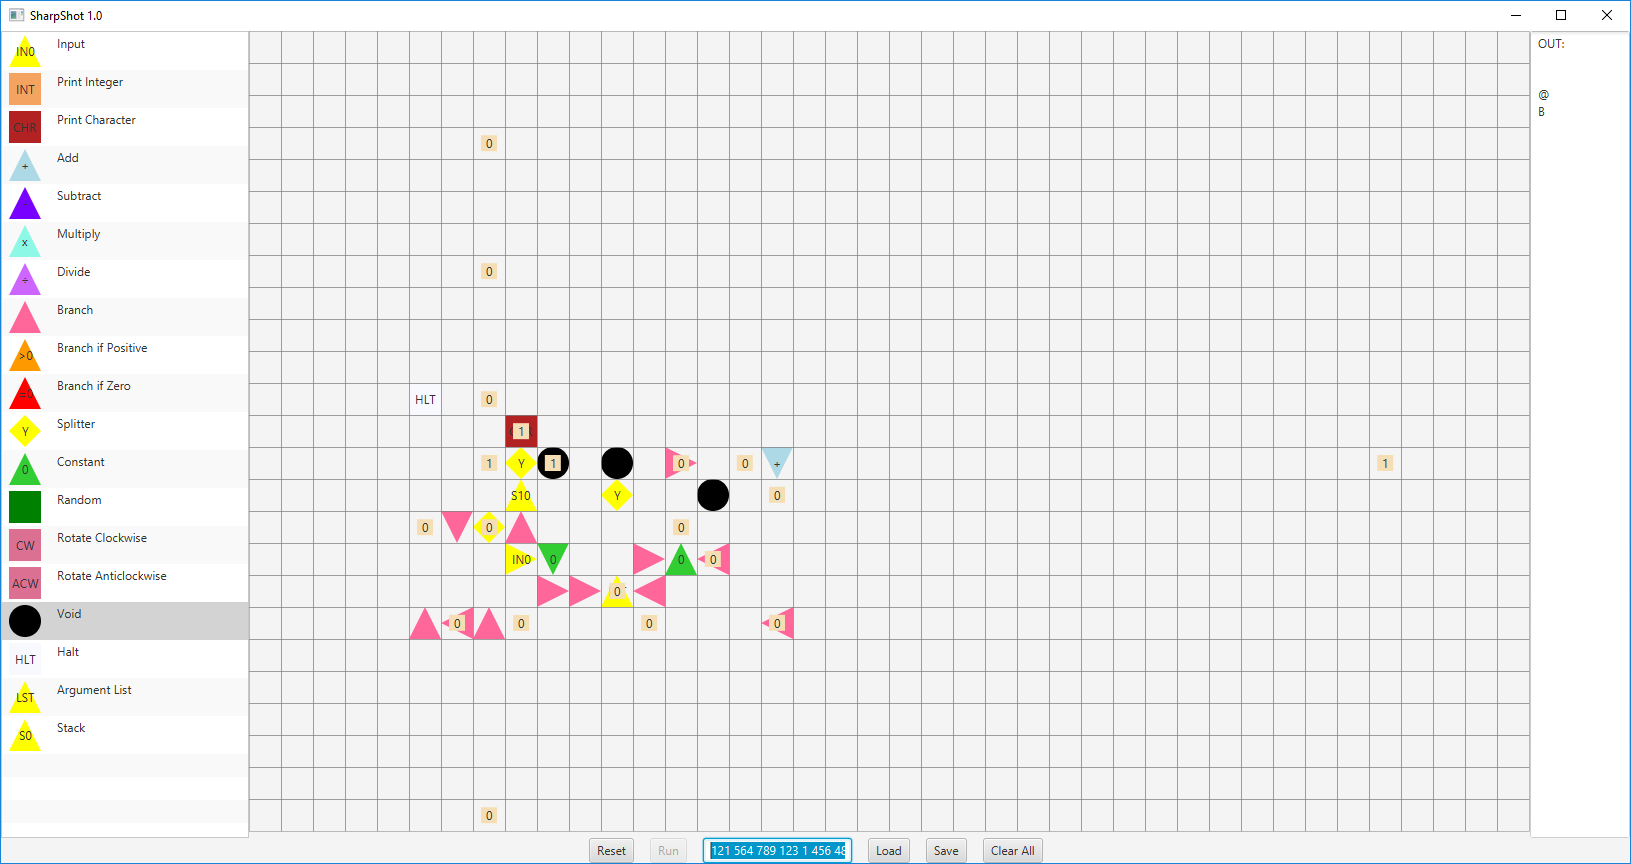
\includegraphics[width=0.9\linewidth]{sharpshot.png}}
		\end{center}
		\vspace{-12pt}
		\href{https://github.com/motherlymuppet/sharpshot}{\textbf{SharpShot} (Oct 2018)}
		
		Created in 24 hours for \href{http://www.durhack.com}{Durhack 2018}. A visual, esoteric programming language where you place nodes on a grid. Each node represents a function, and parameters move around the screen destroying each other when they collide. SharpShot was the overall runner-up from 31 total projects, and won the GitHub prize for best Dev Tool.
		
		\tech{Java} \tech{Kotlin} \tech{Javafx}
		
	\end{minipage}
	\hspace{0.06\textwidth}
	\begin{minipage}{0.40\textwidth}
		
		\begin{center}
			\href{http://www.dsurooms.com}{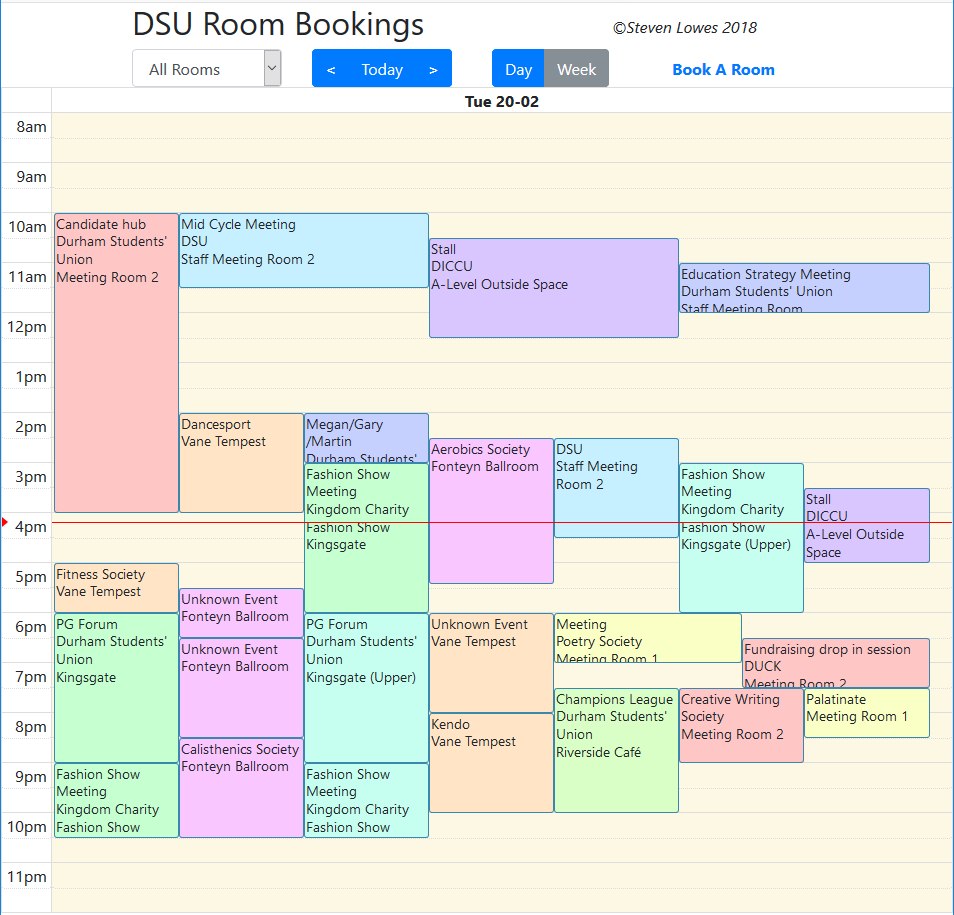
\includegraphics[width=0.9\linewidth]{dsurooms.png}}
		\end{center}
		\vspace{-12pt}
		\href{http://www.dsurooms.com}{\textbf{DSUrooms.com} (Jan 2018)}
		
		Created for Societies Committee, to show when rooms in the Students' Union were booked. Hosted in the cloud using a scraping API created in nodejs. Received very positive feedback from Student Groups, as previously there was no way to know which rooms were booked. Not yet in full release, but in use by a test group.
		
		\tech{NodeJS} \tech{FullCalendar} \tech{Javascript} \tech{JQuery} \tech{RedHat Openshift}
		
		\begin{center}
			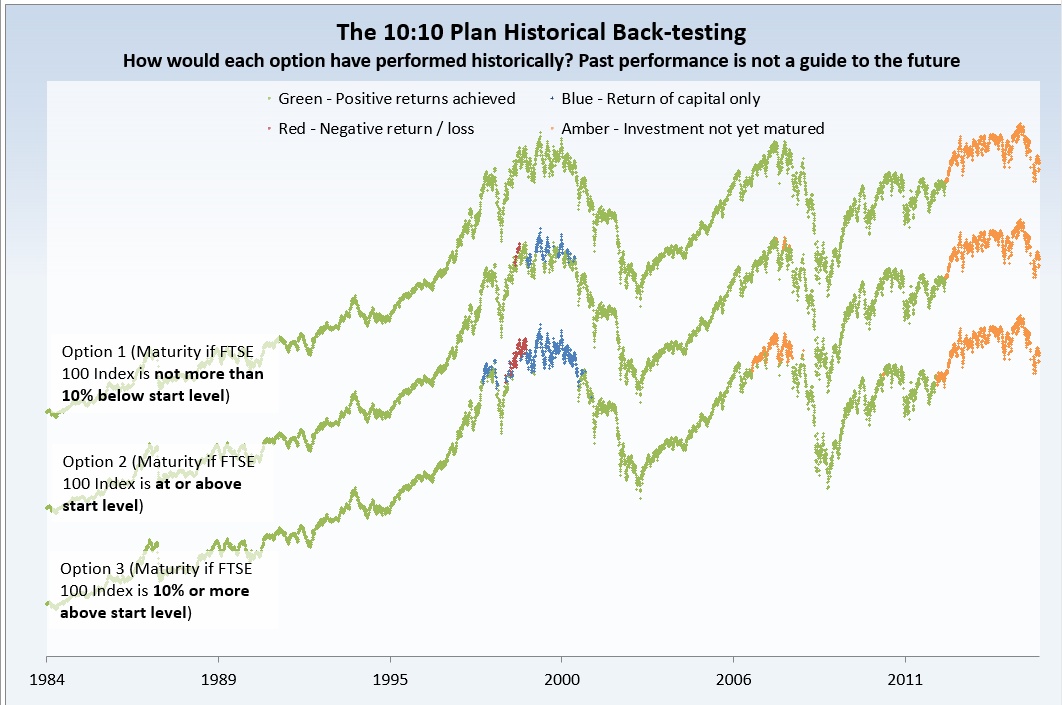
\includegraphics[width=0.9\linewidth]{backtest.png}
		\end{center}
		\vspace{-12pt}
		\textbf{Autocall Backtester} (March 2016)
		
		Created for Lowes Financial Management. Tests a financial product to see how it would have performed historically. This tool allowed the analysis to be performed where previously it was too time consuming. The graphs produced are used in the official product literature and online. The tool also informed the creation of new products, where backtesting revealed them to perform better than expected.
		
		\tech{Java} \tech{Excel} \tech{VBA}
		
	\end{minipage}
	\hspace{0.02\textwidth}
\end{document}